\documentclass{article}
\usepackage{hyperref}
\usepackage{graphicx}

\title{Design Specification \\ USB Content Player}

\author{David M. Dombrowsky \\ 6th Street Radio}

\begin{document}

\maketitle

\section{Goal}

\begin{enumerate}

\item Phase I: Provide a system whereby the client can place DRM
protected content on a USB drive, and end consumer can view but not
easily copy the content.  This replaces the need to, for example,
place video content on an encrypted DVD.  As such, the system needs to
include both the encrypted content {\it and} the player.

\item Phase II: Provide an application that allows clients to manage
their own systems as stated in Phase I.
    \begin{enumerate}
    \item Account authentication
    \item License management.
    \item Generic “support” requests that forward to the client’s 
          technical contact details.
    \end{enumerate}

\item Phase III: Extend functionality to easily offer a facility to
include dynamic content or update content on the drive over an
internet connection.

\end{enumerate}
\newpage
\tableofcontents
\listoffigures
\newpage

\section{Definitions}
Client User - Every USB's Customer/Client company.\\
End User - Client User's end users.\\
Content - Client Users' content to be secured.\\
Data - Client User's data that will not be secured.\\
Package - Encrypted Content\\
App - The USB Package player(s) and the Package.\\
Program - The software that prepares Apps.\\

\section{Requirements}

\begin{enumerate}
\item Work on Windows 7 or greater, and Mac OSX 10 or greater.
\item Support viewing of video using any support \verb+video.js+ format, 
with DRM enabled.
\item Support viewing of PDF files.
\item Support viewing of any image file renderable by the Chromium browser.
\item Prevent user from viewing content files outside of the 
player/viewer included in the device, or when the device is disconnected from 
the end user's computer.
\item Provide a content menu displayed through a Chromium embedded web browser.
\item Allow the user to browse and view content files from within the
Chromium embedded web browser.  This browser is included as part of
the system, and is required to run on all supported operating
systems.\\
(see \url{https://en.wikipedia.org/wiki/Chromium_Embedded_Framework}).  
\item Should “attempt” to forward-prepare for additional phases.
\item Versioning and documentation is essential for understanding
future remote update rollout capability in existing versions already
in use by Every USB’s client’s end users.

\end{enumerate}

\newpage
\section{Design}

Files are presented securely by encrypting them once per individual file,
and then preventing copying at the player/viewer level.  This is demonstrated
in Figure \ref{fig:contentloop}.

\begin{figure}
\centering
\caption{Main Content Loop}
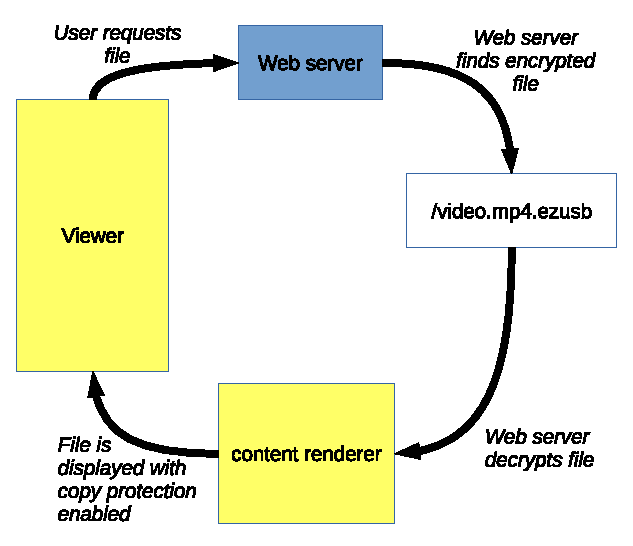
\includegraphics{contentloop.eps}
\label{fig:contentloop}
\end{figure}

To accomplish this, the system has two main parts: the \verb+FILESYSTEM+ 
and the \verb+WEBAPP+, as shown in Figure \ref{fig:mainmods}.

\begin{figure}
\centering
\caption{Main Modules}
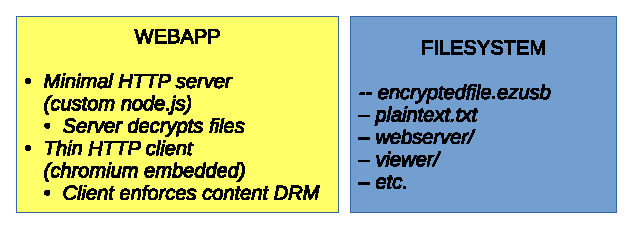
\includegraphics{mainmods.eps}
\label{fig:mainmods}
\end{figure}


\section{Potential Resources}
The following are open source libraries and projects which may be used in the
project, either as a foundation for work or as a guideline.
\begin{itemize}
\item \url{https://electronjs.org/}
\item \url{https://www.nodejs.org}
\item \url{https://www.npmjs.com/package/p3x-aes-folder}
\item \url{https://github.com/tessel/node-usb/tree/master/src}
\item \url{https://github.com/limpkin/mooltiapp}
\item \url{http://janaxelson.com/hidpage.htm}
\item \url{https://github.com/kuscsik/chromiumembedded}
\end{itemize}

\end{document}
